\documentclass{article}
\usepackage[top=0.5in, bottom=0.5in, left=1.25in, right=1.25in]{geometry}

\usepackage{amsmath, array, enumerate, tikz, bm, pgfplots, pgfplotstable, tcolorbox, graphicx, venndiagram, color, colortbl}
\pgfplotsset{compat = newest}
\usepgfplotslibrary{statistics}
\renewcommand{\familydefault}{\sfdefault}
\raggedright
\pagestyle{empty}

\newcounter{example}[section]
\newenvironment{example}[1][]{\refstepcounter{example}\par\medskip
   {\color{red}\textbf{Example~\theexample. #1}}}{\medskip}

\begin{document}

\section*{Measures of Spread}

\begin{tcolorbox}[colframe=orange!70!white, coltitle=black, title=\textbf{Summary}]
\begin{enumerate}
    \item Measures of spread, such as standard deviation, tell us how spread out the data is.
    \item Standard deviation uses the same units as the values in the data set.
\end{enumerate}
\end{tcolorbox}
\vspace{0.75in}

\subsection*{Range}

\begin{tcolorbox}[colframe=green!20!black, colback = green!30!white,title=\textbf{Range}]
The \textbf{range} of a dataset is found by subtracting the minimum value from the maximum value.
\end{tcolorbox}
\vspace{0.75in}

\begin{example}
During a heat wave one summer, I decided to cool off by drinking milkshakes everyday for a week. The number of milkshakes I had each day is shown:	
\begin{center}
9, 2, 7, 10, 3, 4, 12
\end{center}
Find the range for the number of milkshakes I drank that week.
\end{example}
\vspace{0.5in}

A disadvantage of relying solely on the range as a measure of variation is that it is heavily affected by outliers (extreme values).
\vspace{0.5in}

\subsection*{Variance}
\vspace{0.25in}

\begin{tcolorbox}[colframe=green!20!black, colback = green!30!white,title=\textbf{Deviation from the Mean}]
The \textbf{deviation from the mean} refers to how far a data value, $x$, is from the mean; found by \[x - \text{mean}\]
\end{tcolorbox}

Deviation can be positive, negative, or zero.
\vspace{0.5in}

\begin{example}
Find the mean of the following gas prices: 
\begin{center}
\$3.25, \$3.40, \$3.21, \$3.38
\end{center}
\end{example}

\newpage 

We can think of the mean as a ``balancing point'' for our data set:	\vspace{11pt}
\begin{center}
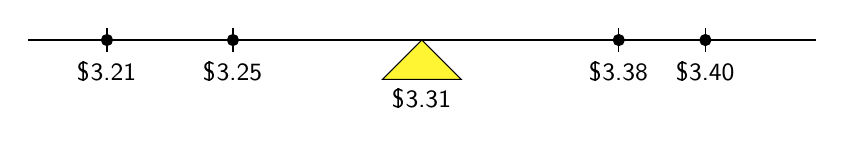
\begin{tikzpicture}
\draw (-5,0) -- (5,0);
\draw [fill=yellow!80] (0,0) -- (-0.5,-0.5) -- (0.5,-0.5) -- cycle;
\node at (0,-0.5) [below] {\small\$3.31};
\draw (-4,0.15) -- (-4,-0.15) node [below] {\small\$3.21};
\draw [color=black, fill] (-4,0) circle [radius=2pt];
\draw (-2.4,0.15) -- (-2.4,-0.15) node [below] {\small\$3.25};
\draw [color=black, fill] (-2.4,0) circle [radius=2pt];
\draw (3.6,0.15) -- (3.6,-0.15) node [below] {\small\$3.40};
\draw [color=black, fill] (3.6,0) circle [radius=2pt];
\draw (2.5,0.15) -- (2.5,-0.15) node [below] {\small\$3.38};
\draw [color=black, fill] (2.5,0) circle [radius=2pt];
\end{tikzpicture}
\end{center}
\vspace{0.25in}

Each data point has a deviation (or \emph{distance}) from the mean.
\vspace{0.5in}

\begin{example}
Calculate each data point's deviation from the mean.	\newline\\	
\$3.25, \$3.40, \$3.21, \$3.38	\qquad (Mean: \$3.31)
\end{example}
\vspace{1.25in}

\begin{example}
Find the mean of the deviations from the previous example.
\end{example}
\vspace{1.5in}

\begin{itemize}
    \item Positive deviations will always ``cancel out" negative deviations.
    \item Two possible remedies:
    \begin{itemize}
        \item Take absolute value of deviations
        \item Square the deviations
    \end{itemize}
    \item Absolute values will lead us to \textit{mean absolute deviation}.
    \item For future calculations, squaring is the better choice.
\end{itemize}
\vspace{1.25in}

\begin{example}
Square each of the deviation gas prices and then find the mean of the squared deviations.
\end{example}

\newpage 

The result of the previous example is known as the {\color{blue}\textbf{population variance}} and is denoted by 

\[\sigma^2\] 

\vspace{0.25in}

Like the mean, variance also has a {\color{red}\textbf{sample variance}} and is denoted 

\[s^2\]
\vspace{0.5in}

\textsc{Population vs. Sample Variance}

\begin{itemize}
    \item Sample variance $\longrightarrow$ divide by \emph{one less} than then number of observations ({\color{blue}\textbf{degrees of freedom}}).
    \item Sum of the deviations \textbf{must} be 0.
    \begin{itemize}
    \item In a data set with 4 entries, the first 3 entries can be any number we want.
    \item The final value \underline{must} make it so that the sum of the deviations from the mean equals 0.
    \end{itemize}
\end{itemize}
\vspace{0.5in}

\begin{center}
\setlength{\extrarowheight}{7pt}
\begin{tabular}{c|c}
\textbf{Population Variance} & \textbf{Sample Variance} \\ \hline
$\sigma^2 = \frac{\sum (x_i-\mu)^2}{N}$	&	$s^2 = \frac{\sum (x_i-\bar{x})^2}{n-1}$
\end{tabular}
\end{center}

\vspace{0.25in}

\emph{Note}: Variance always gives us squared units of measurement.
\vspace{0.75in}

\begin{tcolorbox}[colframe=green!20!black, colback = green!30!white,title=\textbf{Standard Deviation}]
The \textbf{standard deviation} is the square root of variance.
\[
\text{Standard Deviation} = \sqrt{\text{Variance}}
\]
\end{tcolorbox}
\vspace{0.25in}

\[\sigma = \sqrt{\frac{\sum (x_i-\mu)^2}{N}} \quad \text{and} \quad s = \sqrt{\frac{\sum (x_i-\bar{x})^2}{n-1}}\]
\vspace{0.5in}

\textsc{Properties of Standard Deviation}:

\begin{itemize}
	\item It's a measure of how much (on average) the data values deviate from the mean.
	\item Can be positive or 0 \underline{only}.
	\item Like the mean, it can be greatly affected by extreme values (outliers).
	\item The units are the same as those in the data set.
	\item Less and less differences between population and sample s.d. with larger sample sizes.
\end{itemize}

\newpage 

\begin{example}
Find population AND sample standard deviations of the gas prices.
\end{example}
\vspace{2in}

\emph{Usually}, data values will be within 2 standard deviations of the mean.
\vspace{1in}

\begin{example}
The mean price of gas one day was \$3.58 with a standard deviation of \$0.33. What interval would represent a ``usual" price of gas?
\end{example}
\end{document}
